\documentclass{article}

% if you need to pass options to natbib, use, e.g.:
%     \PassOptionsToPackage{numbers, compress}{natbib}
% before loading neurips_2020

% ready for submission
 %\usepackage{neurips_2020}

% to compile a preprint version, e.g., for submission to arXiv, add add the
% [preprint] option:
\usepackage[preprint]{neurips_2020}

% to compile a camera-ready version, add the [final] option, e.g.:
%\usepackage[final]{neurips_2020}

% to avoid loading the natbib package, add option nonatbib:
%\usepackage[nonatbib]{neurips_2020}

\usepackage[utf8]{inputenc} % allow utf-8 input
\usepackage[T1]{fontenc}    % use 8-bit T1 fonts
\usepackage{hyperref}       % hyperlinks
\usepackage{url}            % simple URL typesetting
\usepackage{booktabs}       % professional-quality tables
\usepackage{amsfonts}       % blackboard math symbols
\usepackage{nicefrac}       % compact symbols for 1/2, etc.
\usepackage{microtype}      % microtypography

% Added packages
\usepackage{amsmath,amssymb}

\title{Your Project Title (e.g. Replication: Policy Optimization with Demonstrations)}

% The \author macro works with any number of authors. There are two commands
% used to separate the names and addresses of multiple authors: \And and \AND.
%
% Using \And between authors leaves it to LaTeX to determine where to break the
% lines. Using \AND forces a line break at that point. So, if LaTeX puts 3 of 4
% authors names on the first line, and the last on the second line, try using
% \AND instead of \And before the third author name.

\author{%
  Author names\\
  Department of Computer Science\\
  National Yang Ming Chiao Tung University\\
  \texttt{\{xxx, yyy, zzz\}@nycu.edu.tw}
}

\begin{document}

\maketitle


\section{Problem Overview}
\label{section:intro}
This paper introduces a new softmax operator during action selection, which can be used in a SARSA algorithm that computes a Boltzmann policy with a state-dependent temperature parameter. The algorithm is convergent and serves as an alternative to the original Boltzmann policy. The main research problem that is tackled by the paper is that all the common using softmax operator are not idea operator. Some are not non-expansion, some are not differentiable. Hence, The author proposed mellowmax softmax operator that is proved to be an idea operator and generate a well trade-off between exploration and exploitation during action selection.

\section{Background and The Algorithm}
\label{section:algorithm}
An ideal softmax operator is a parameterized set of operators that:
\begin{itemize}
\item has parameter settings that allow it to approximate maximization arbitrarily accurately to perform reward-seeking behavior;
\item is a non-expansion for all parameter settings ensuring convergence to a unique fixed point;
\item is differentiable to make it possible to improve via gradient-based optimization; and
\item avoids the starvation of non-maximizing actions.
\item Let $X = x_{1},...,x_{n}$ be a vector of values. We define the following operators:
\end{itemize}

% \textbf{Lemma 2}
\begin{figure}[H] %H为当前位置,!htb为忽略美学标准,htbp为浮动图形
\centering %图片居中
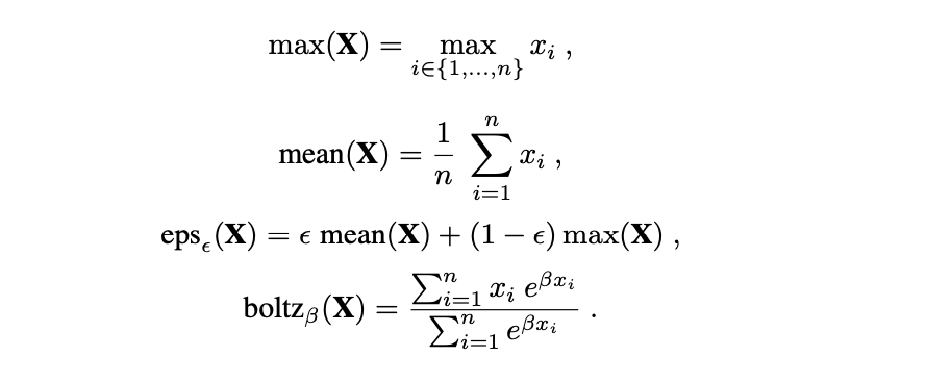
\includegraphics[width=0.7\textwidth]{algorithm.eps} %插入图片,[]中设置图片大小,{}中是图片文件名
% \caption{A list of not ideal softmax operator} %最终文档中希望显示的图片标题
% \label{Fig.main2} %用于文内引用的标签

\end{figure}
The Boltzmann operator $boltz_{\beta}(X)$ is differentiable. It also approximates max as $\beta $→ $\infty$and mean as $\beta $→ $0$ . However, it is not a non-expansion operator, and therefore, the lack of the non-expansion property leads to multiple fixed points and ultimately a misbehavior in learning and planning.
\newpage
\textbf{MellowMax}
\newline\newline
Author presents a new softmax operator that is similar to the Boltzmann operator yet is a non-expansion operator. Author also proves several critical properties of this new operator, introduce a new softmax policy, and present empirical results. The alternative mellowmax softmax operator is defined as follows:
\begin{figure}[H] %H为当前位置,!htb为忽略美学标准,htbp为浮动图形
\centering %图片居中
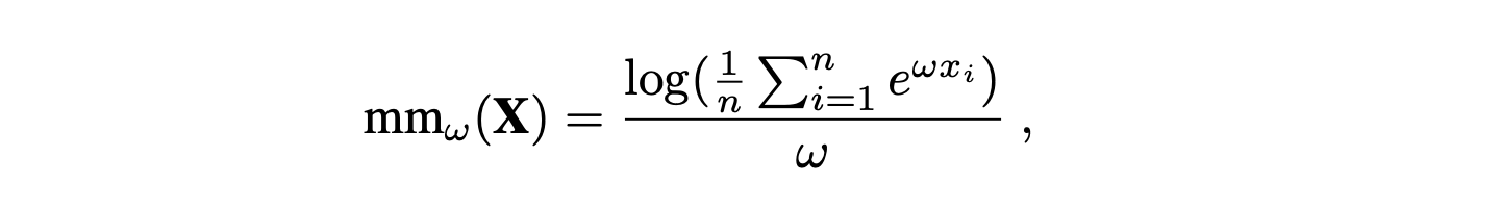
\includegraphics[width=0.7\textwidth]{mel.eps} %插入图片,[]中设置图片大小,{}中是图片文件名
% \caption{mellowmax softmax operator} %最终文档中希望显示的图片标题
% \label{Fig.main2} %用于文内引用的标签

\end{figure}

Author proves that $mm\omega$ is a non-expansion operator, and therefore, GVI and SARSA under $mm\omega$ are guaranteed to converge to a unique fixed point.
Furthermore, the operator acts more and more like pure maximization as the value of $\omega$ is increased. Conversely, as $\omega$ goes to $-\infty$, the operator approaches the minimum.
And as ${\omega}$ gets closer to zero, $mm_{\omega}(x)$ approaches the
mean of the values in $X$.


\textbf{Mellowmax Policy}
\newline\newline
Author formally defines the maximum entropy mellowmax policy of a state $s$ as:
\begin{figure}[H] %H为当前位置,!htb为忽略美学标准,htbp为浮动图形
\centering %图片居中
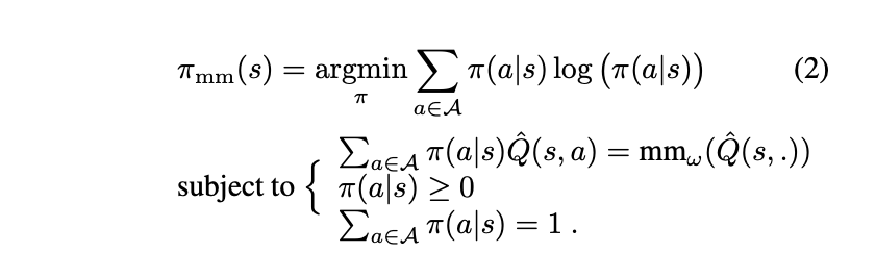
\includegraphics[width=0.7\textwidth]{entropy.eps} %插入图片,[]中设置图片大小,{}中是图片文件名
% \caption{mellowmax softmax operator} %最终文档中希望显示的图片标题
% \label{Fig.main2} %用于文内引用的标签
\end{figure}

After using the method of Lagrange multipliers to solve this system of equations, the probability of taking an action under the maximum entropy mellowmax policy has the form:
\begin{figure}[H] %H为当前位置,!htb为忽略美学标准,htbp为浮动图形
\centering %图片居中
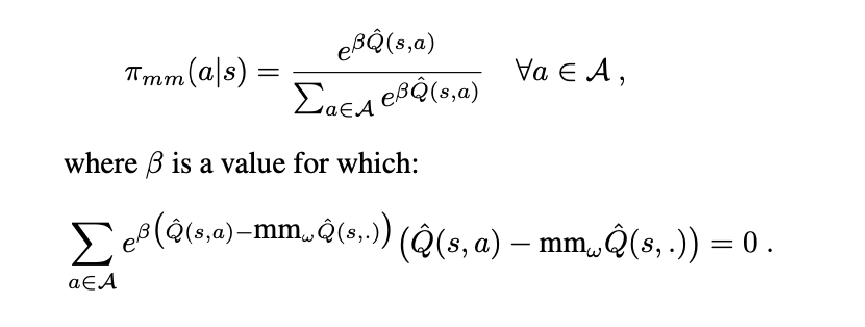
\includegraphics[width=0.7\textwidth]{result.eps} %插入图片,[]中设置图片大小,{}中是图片文件名
% \caption{mellowmax softmax operator} %最终文档中希望显示的图片标题
% \label{Fig.main2} %用于文内引用的标签
\end{figure}

The argument for the existence of a unique root is simple. As $\beta$ → $\infty$, the term corresponding to the best action dominates, and so, the function is positive. Conversely, as $\beta$ → $-\infty$, the term corresponding to the action with lowest utility dominates, and so the function is negative. Finally, by taking the derivative, it is clear that the function is monotonically increasing, allowing us to conclude that there exists only a single root. Therefore, we can find $\beta$ easily using any root-finding algorithm. 
\newline\newline
This policy has the same form as Boltzmann softmax, but with a parameter $\beta$ whose value depends indirectly on $\omega$. This mathematical form arose not from the structure of $mm\omega$, but from maximizing the entropy. One way to view the use of the mellowmax operator, then, is as a form of Boltzmann policy with a temperature parameter chosen adaptively in each state to ensure that the non-expansion property holds.

\section{Detailed Implementation}
\label{section:implementation}
Please explain your implementation in detail. You may do this with the help of pseudo code or a figure of system architecture. Please also highlight which parts of the algorithm lead to the most difficulty in your implementation.




\section{Empirical Evaluation}
\label{section:evaluation}



% =======================================================================

\subsection{Simple MDP and Random MDPs}

The author of this paper construct a handcrafted simple MDP, as shown in figure\ \ref{fig:simple_mdp}.
It is composed of two states $s_1$ and $s_2$. State $s_2$ is a terminal state, and only $s_1$ is a non-terminal state.
The edges are labeled with a transition probability (unsigned) and a reward number (signed). Discount factor $\gamma=0.98$.
State $s_1$ has two actions a and b. In the following simple MDP experiments, we mainly focus on the Q value of a and b.

% {\begin{wrapfigure}{l}{0.25\textwidth}
%     \centering    
%     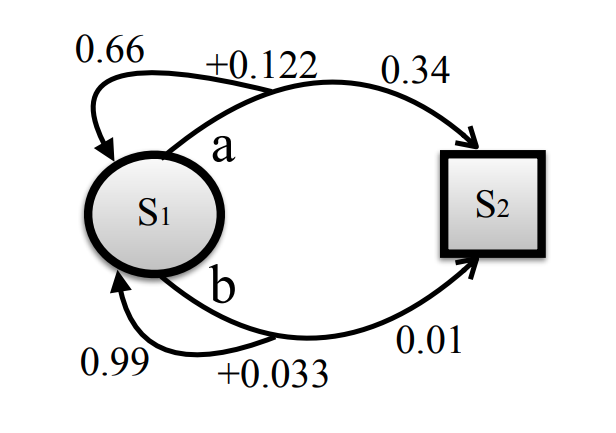
\includegraphics[width=0.25\textwidth]{simple_mdp_fig.png}
%     \caption{Simple MDP Settings}\label{fig:simple_mdp}
% \end{wrapfigure}}

\begin{figure}[H]
    \centering
    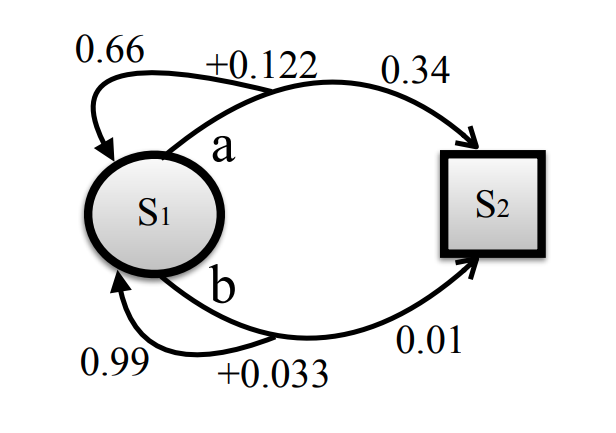
\includegraphics[width=0.25\textwidth]{simple_mdp_fig.png}
    \caption{Simple MDP}\label{fig:simple_mdp}
\end{figure}

% =======================================================================
\subsubsection{Simple MDP\ -\ SARSA}

Figure\ \ref{fig:simple_mdp_sarsa} shows the results of SARSA (algorithm) running 2000 episodes in this MDP. 
The blue and green lines depict the Q-values for both actions in each episode. 
Boltzmann curves have significantly larger oscillations. 
Its swing range is around 0.3 to 0.4, while the Q value of the Mellowmax curve is
relatively stable; its swing range is around 0.2.

{\centering
\begin{figure}[H]
\begin{tabular}{cc}
\begin{subfigure}{0.45\textwidth}\centering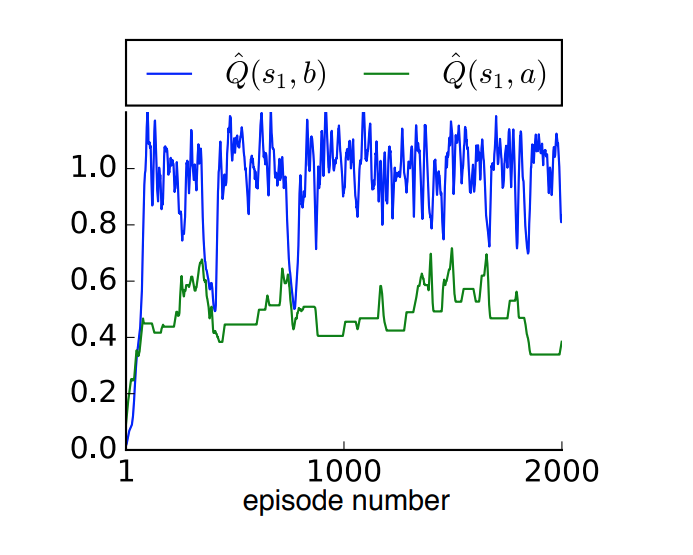
\includegraphics[width=0.9\columnwidth, height=5cm]{SARSA_Boltz_paper.png}\caption{Boltz (paper)}\end{subfigure}&
\begin{subfigure}{0.45\textwidth}\centering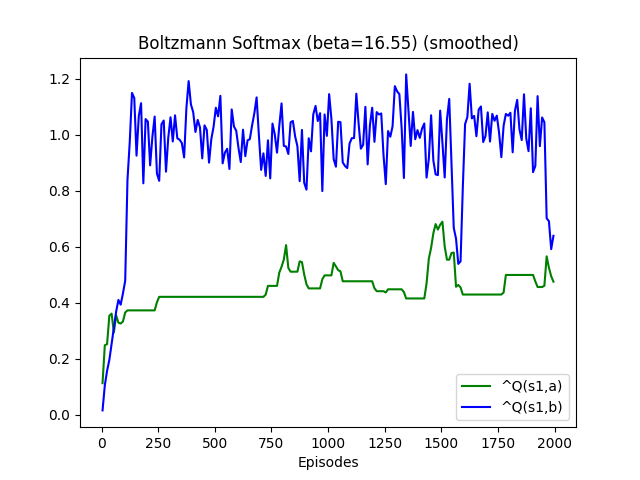
\includegraphics[width=0.9\columnwidth, height=5cm]{SARSA_sampleMDP_Boltzmann Softmax_smoothed.png}\caption{Boltz (replication)}\end{subfigure}\\
\newline
\begin{subfigure}{0.45\textwidth}\centering
\includegraphics[width=0.9\columnwidth, height=5cm]{white.png}\caption{Mellowmax (paper does not has this)}\end{subfigure}&
\begin{subfigure}{0.45\textwidth}\centering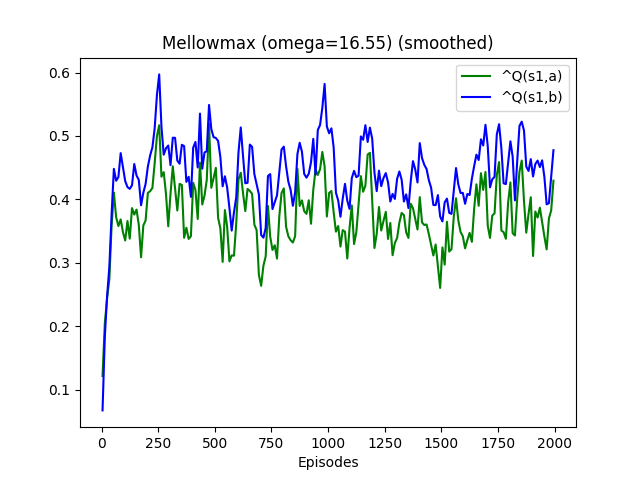
\includegraphics[width=0.9\columnwidth, height=5cm]{SARSA_sampleMDP_Mellowmax_smoothed.png}\caption{Mellowmax (our)}\end{subfigure}\\
\end{tabular}
\caption{SARSA with bolz/mm policy ($\beta=16.55$, $\omega=16.55$)}\label{fig:simple_mdp_sarsa}
\end{figure}}

% =======================================================================
\subsubsection{Simple MDP\ -\ GVI}

Compared with value iteration, GVI doesn not restrict the way to compute 
$\otimes Q(s',\cdot)$. Max, Boltzmann Softmax, Mellowmax, and other operators can be used as an operator.
(For more detail of GVI, please refer to\cite{littman1996generalized}.)

Figure\ \ref{fig:simple_mdp_gvi_paper} (from paper) demonstrates the GVI result of
Boltzmann Softmax and Mellowmax. An arrow is the updating direction and step size of a Q pair.
Black points are the convergence fixed points. As we can see, in this case, there are two convergence points of Boltzmann Softmax's,
while Mellowmax has only one convergence point. 

Besides, the arrows on the figure tell us that the updating size is small 
when the Q pair locates at the position near the convergence point.
This phenomenon is more obvious at the position between two convergence points especially.
Thus, when there are more than one fixed points, 
the value may stay in the area between two convergence points with a tiny updating size, 
needing more iterations to reach a convergence point.

Boltzmann Softmax does not have the non-expansion property, 
so it is not under the convergence guarantee from the original GVI paper (\cite{littman1996generalized}). 
If there are > 1 convergence fixed points, the noise may drive it to swing 
between different points and lead to instability.

{\centering
\begin{figure}[H]
\begin{tabular}{cc}
\begin{subfigure}{0.45\textwidth}\centering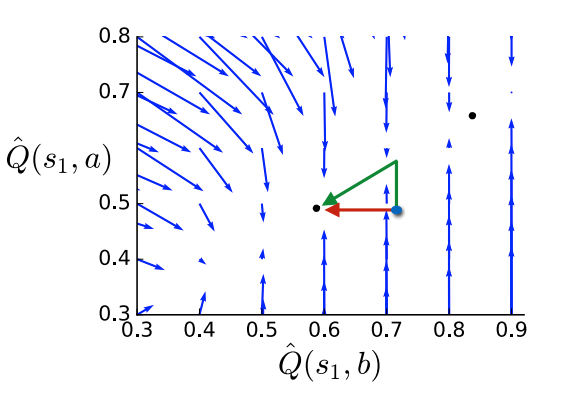
\includegraphics[width=0.95\columnwidth, height=5cm]{simpleMDP_GVI_boltz_paper.png}\caption{Boltz (paper)}\end{subfigure}&
\begin{subfigure}{0.45\textwidth}\centering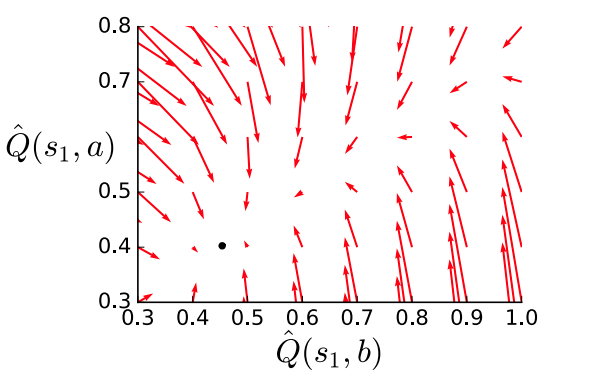
\includegraphics[width=0.95\columnwidth, height=5cm]{simpleMDP_GVI_mm_paper.png}\caption{Mellowmax (paper)}\end{subfigure}\\
\end{tabular}
\caption{Paper's GVI with bolz/mm policy ($\beta=16.55$, $\omega=16.55$)}\label{fig:simple_mdp_gvi_paper}
\end{figure}}


Figure\ \ref{fig:simple_mdp_gvi_our_bolz} is our replication of GVI with Boltzmann Softmax policy under different hyper-parameter $\beta$.
A blue arrow displays the first updating direction and relative size  of one initial point.
A green arrow displays the direction and relative updating size from starting point to convergence point.
A red/balck point is a convergence fixed point.
A range of $\beta$ is tried, and we find under some $\beta$, there more than one convergence points as the figures shown.

{\centering
\begin{figure}[H]
\begin{tabular}{ccc}
\begin{subfigure}{0.33\textwidth}\centering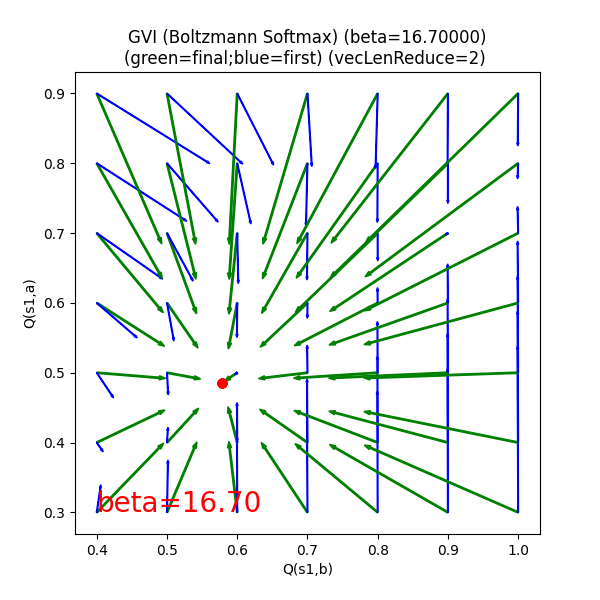
\includegraphics[width=0.9\columnwidth, height=4.5cm]{our_simple_boltz1.png}\caption{$\beta=16.7$}\end{subfigure}&
\begin{subfigure}{0.33\textwidth}\centering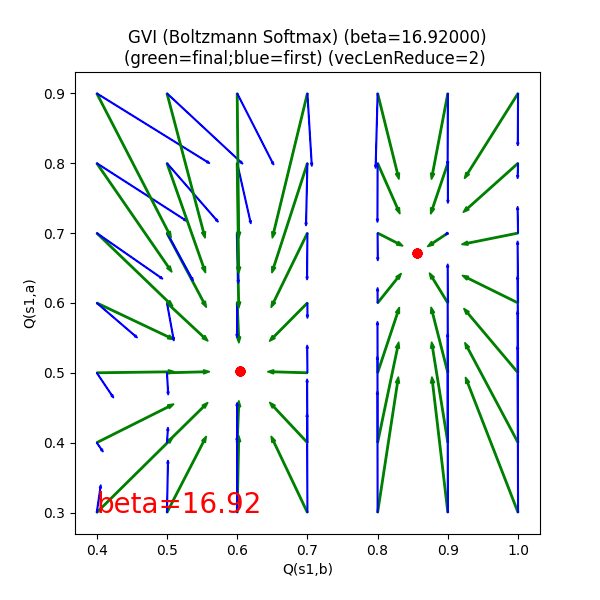
\includegraphics[width=0.9\columnwidth, height=4.5cm]{our_simple_boltz2.png}\caption{$\beta=16.92$}\end{subfigure}&
\begin{subfigure}{0.33\textwidth}\centering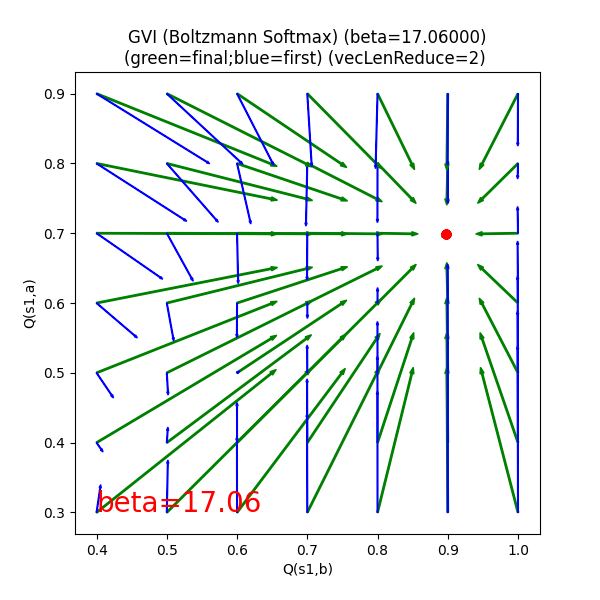
\includegraphics[width=0.9\columnwidth, height=4.5cm]{our_simple_boltz3.png}\caption{$\beta=17.06$}\end{subfigure}\\
\end{tabular}
\caption{Our Boltzmann GVI replication (boltz)}\label{fig:simple_mdp_gvi_our_bolz}
\end{figure}}

In conparison, Mellowmax does not show that it has more than one fixed points in our experiment.
It's relative stable. We try to change $\omega$ from around 16.7 to 17, and 
the fixed point only move for a very small distance and stay near the point, as figure\ \ref{fig:simple_mdp_gvi_our_mm} displays.

{\centering
\begin{figure}[H]
\begin{tabular}{ccc}
\begin{subfigure}{0.33\textwidth}\centering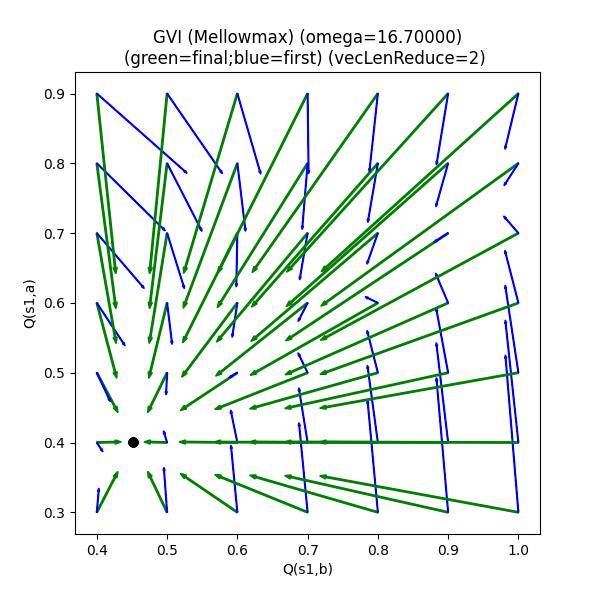
\includegraphics[width=0.9\columnwidth, height=4.5cm]{our_simple_mdp_gvi_mm167.png}\caption{$\beta=16.7$}\end{subfigure}&
\begin{subfigure}{0.33\textwidth}\centering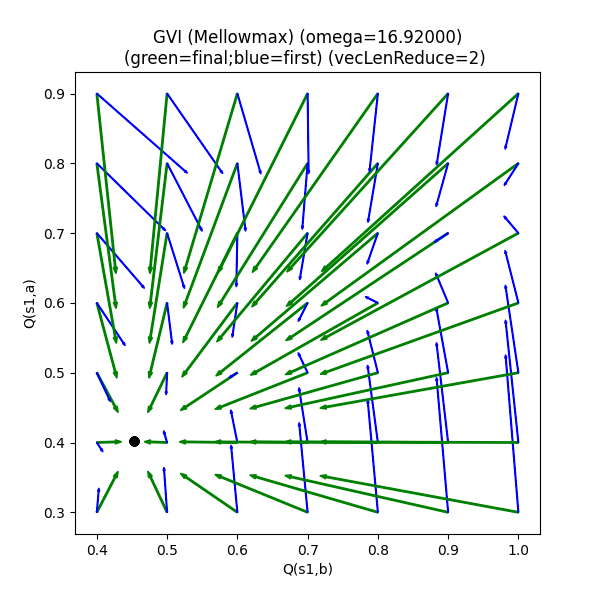
\includegraphics[width=0.9\columnwidth, height=4.5cm]{our_simple_mdp_gvi_mm1692.png}\caption{$\beta=16.92$}\end{subfigure}&
\begin{subfigure}{0.33\textwidth}\centering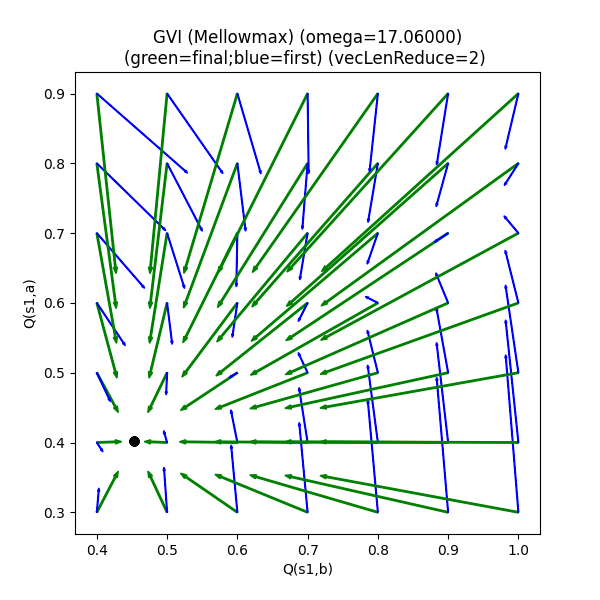
\includegraphics[width=0.9\columnwidth, height=4.5cm]{our_simple_mdp_gvi_mm176.png}\caption{$\beta=17.06$}\end{subfigure}\\
\end{tabular}
\caption{Our Boltzmann GVI replication (mm)}\label{fig:simple_mdp_gvi_our_mm}
\end{figure}}

The exact value of beta when it does not converge at only one point 
derived by us is not precisely equivalent to that shown on paper. 
But both of it show GVI with Boltzmann Softmax under a period of $\beta$ 
near 16.7 converge at more than one points.


The following figure is from paper and it is obtained by trying different betas for GVI using the Boltzmann Softmax policy. 
Similar to the results in Figure\ \ref{fig:simple_mdp_gvi_paper} and\ \ref{fig:simple_mdp_gvi_our_bolz},
there are more than one convergence fixed point under some $\beta$.

\begin{figure}[H]
    \centering
    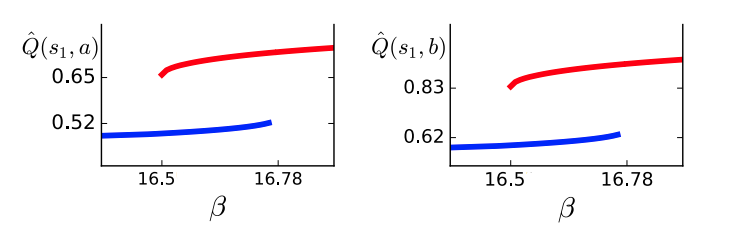
\includegraphics[width=0.7\textwidth]{simpleMDP_boltz_paper_diff_beta.png}
    \caption{Number of different fixed points under different $\beta$ (GVI with boltz)}\label{fig:simple_mdp_boltz_paper_diff_beta}
\end{figure}

Figure\ \ref{fig:simple_mdp_gvi_our_diff_beta} is our result. 
Subfigure\ \ref{subfig:our_diff_beta_boltz} shows fixed points of GVI using Boltzmann Softmax 
under different $\beta$. Although the precise value is not completely the same as figure\ \ref{fig:simple_mdp_boltz_paper_diff_beta},
it demonstrates the same result as figure\ \ref{fig:simple_mdp_boltz_paper_diff_beta}-there are more than one convergence fixed points under some $\beta$.

We make an additional subfigure\ \ref{subfig:our_diff_beta_mm} to show Mellowmax's result. 
Akin to what figure 5 shows, the fixed point of Mellowmax doesn't change a lot under different hyper-parameter $\omega$.
By comparison, it can be found that the convergence point of Boltzmann Softmax is more sensitive to hyperparameter tuning, 
while the convergence point of Mellomax is less affected by hyperparameter changes.

\begin{figure}[H]
\centering
\begin{tabular}{cc}
\begin{subfigure}{0.45\textwidth}\centering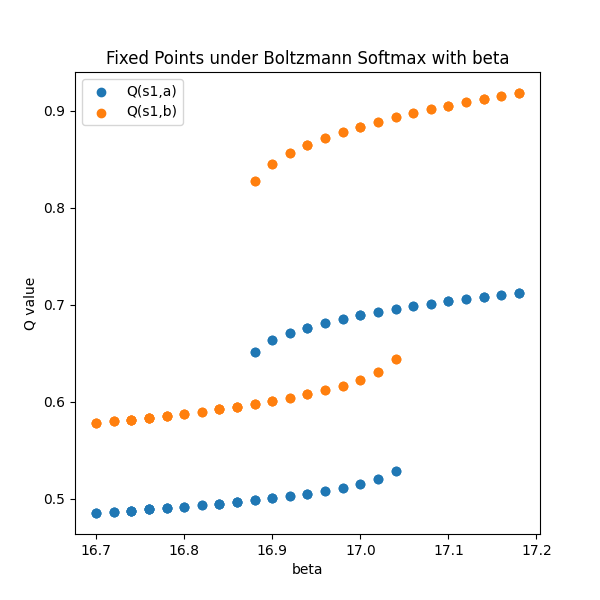
\includegraphics[width=0.9\columnwidth]{simpleMDP_boltz_our_diff_beta.png}\caption{Boltzmann Softmax}\label{subfig:our_diff_beta_boltz}\end{subfigure}&
\begin{subfigure}{0.45\textwidth}\centering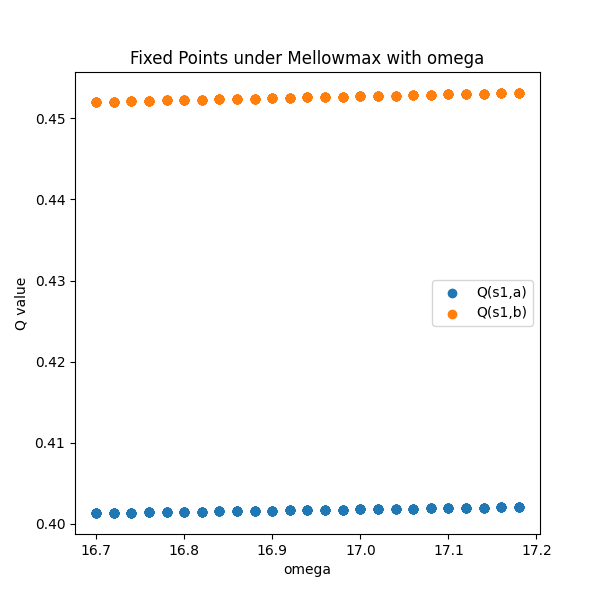
\includegraphics[width=0.9\columnwidth]{simpleMDP_mm_our_diff_beta.png}\caption{Mellowmax}\label{subfig:our_diff_beta_mm}\end{subfigure}\\
\end{tabular}
\caption{Our replication}\label{fig:simple_mdp_gvi_our_diff_beta}
\end{figure}



% =======================================================================
\subsubsection{Random MDPs}

The experiments discussed so far were run in a handcrafted MDP environment. 
To see if these properties also exist under natural conditions, 
the paper conducts experiments on random MDPs to observe if 
randomly generated MDPs using these two policies for GVI also have these properties.

Figure\ \ref{fig:randomMDP_paper} is the result from paper. 
It tries 200 MDPs. No termination means the GVI cannot converge within a predefined max number
of iterations. Boltzman Softmax has these results: non-termination and >1 fixed points, 
while Mellowmax does not. In addition, Boltzmann Softmax requires more iterations on average to converge.

\begin{figure}[H]
    \centering
    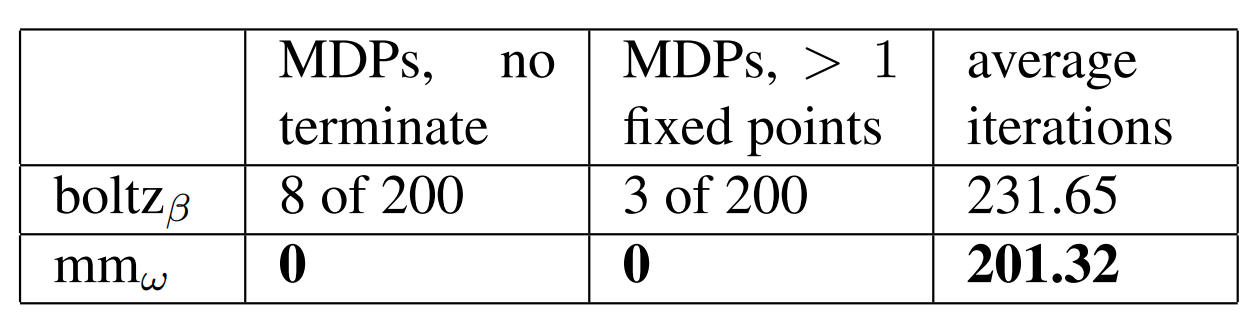
\includegraphics[width=0.5\textwidth]{randomMDP_paper.png}
    \caption{Random MDPs (paper). Max iteration is set 1000.}\label{fig:randomMDP_paper}
\end{figure}

Figure\ \ref{fig:randomMDP_paper} is our result.
The way we construct random MDPs is a little different from the paper. 
See Algorithm\ \ref{alg:RandomMDP-GVI} for details. We tried 200 MDPs; 100 trials were run for each MDP. 
The values of no-termination and average iteration in the figure are the results of averaging all MDPs' all trials.
The values of > 1 fixed points are the results of averaging all MDPs' number.
It can be seen that it presents the same characteristics as in Figure\ \ref{fig:randomMDP_paper}.

\begin{figure}[H]
    \centering
    \begin{tabular}{ |c|c|c|c| } 
     \hline
     { }  & avg \# no terminate & avg \# > 1 fixed points & avg interation\\ 
     \hline
     $\text{boltz}_\beta$ & 0.00675 & 0.03 & 1085.0973\\ 
     \hline
     $\text{mm}_\omega$ & 0 & 0 & 1048.794 \\ 
     \hline
    \end{tabular}
    \caption{Random MDPs (our). Max iteration is set 2000. There are 200 MDPs tried; each MDP has 100 trials.}\label{fig:randomMDP_our}
\end{figure}


\subsubsection{How to determin wheter > 1 fixed points?}
{Note that the paper doesn't explain how they determine whether > 1 fixed points. 
The approach we use to decide if > 1 fixed points is to sample different initial Q values 
in each trial to see if there are different fixed points in all trials. 
That's why we run 100 trials for each MDP in figure \ref{fig:randomMDP_our}. 
Although getting no > 1 fixed points by this method doesn't means it must actually have no > 1 fixed points, 
at least, we can derive it has a higher probability or less probability to have > 1 fixed points. 
For example, in our experiment result, Mellowmax never has > 1 fixed points among all trials, 
while Boltzmann has. We can infer that Boltzmann has at least a higher probability to have > 1 fixed points than Mellowmax.
}\label{randomMDP_finding_fixed_points_issue}


% ###########################################################################
% ###########################################################################

\subsection{Taxi Domain}

Sarsa with epsilon-greedy, learning rate $\alpha = 0.1$, discount factor $\gamma = 1 $, we test different $\epsilon$ values, $\epsilon = 0.05, 0.1, 0.2, 0.3, 0.5$, and the result are averaged over 6 independent runs, each consisting of 100000 time steps.

Sarsa with Boltzmann softmax, learning rate $\alpha = 0.1$, discount factor $\gamma = 1 $, we test different $\beta$ values, $\beta = 0.5, 1, 2, 3, 5, 10$, and the result are averaged over 6 independent runs, each consisting of 100000 time steps.

Sarsa with Mellowmax softmax, learning rate $\alpha = 0.1$, discount factor $\gamma = 1 $, we test different $\omega$ values, $\omega = 0.5, 1, 2, 3, 5, 50$, and the result are averaged over 6 independent runs, each consisting of 10000 time steps. We know that when $\omega \to \infty$, Mellowmax will behave like max operator, and we set $\omega$ to 50 so that the result will similar to the paper and show that phenomenon.

{\centering
\begin{figure}[H]
\begin{tabular}{ccc}
\begin{subfigure}{0.32\textwidth}\centering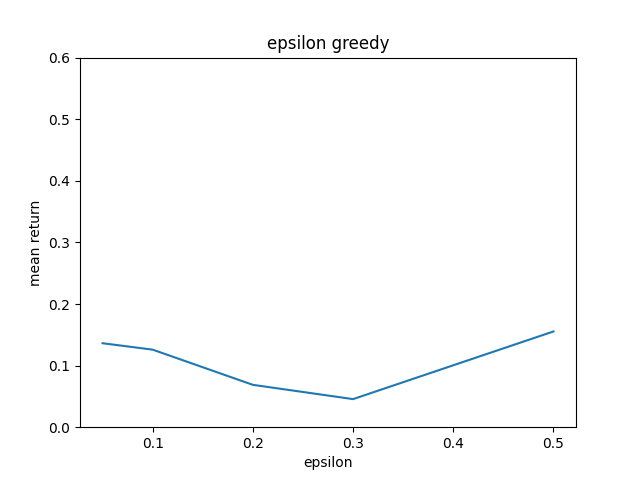
\includegraphics[width=0.98\columnwidth, height=4cm]{taxi_1.png}\caption{Boltz (paper)}\end{subfigure}&
\begin{subfigure}{0.32\textwidth}\centering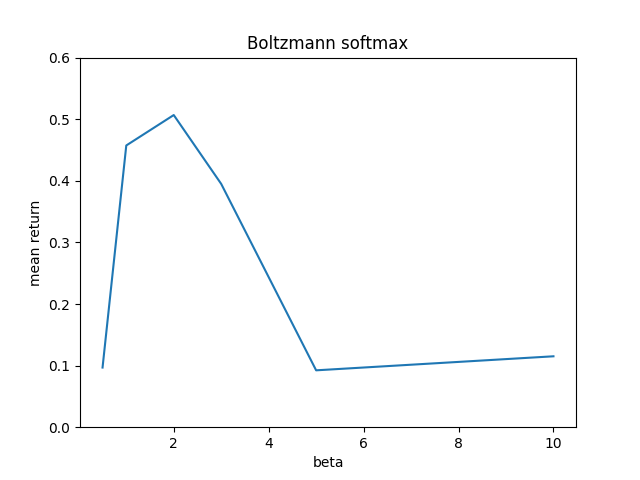
\includegraphics[width=0.98\columnwidth, height=4cm]{taxi_2.png}\caption{Boltz (paper)}\end{subfigure}&
\begin{subfigure}{0.32\textwidth}\centering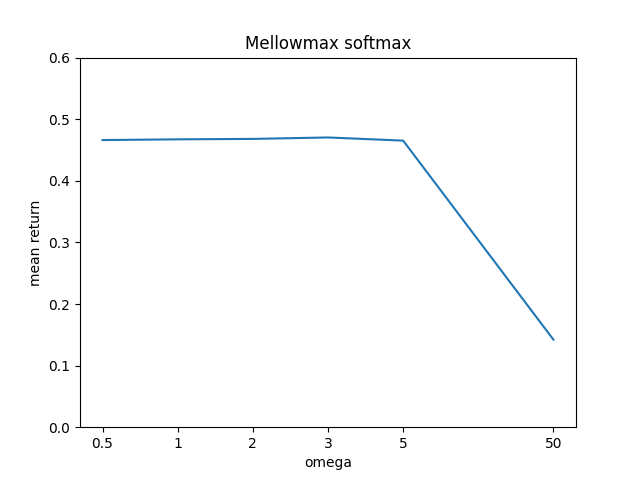
\includegraphics[width=0.98\columnwidth, height=4cm]{taxi_3.png}\caption{Boltz (paper)}\end{subfigure}\\
\end{tabular}
\caption{Taxi domain result}
\end{figure}}

% ###########################################################################
% ###########################################################################


\subsection{Lunar Lander Domain}
\subsection*{Experiment Results}
The paper's results:\\
\begin{center}
    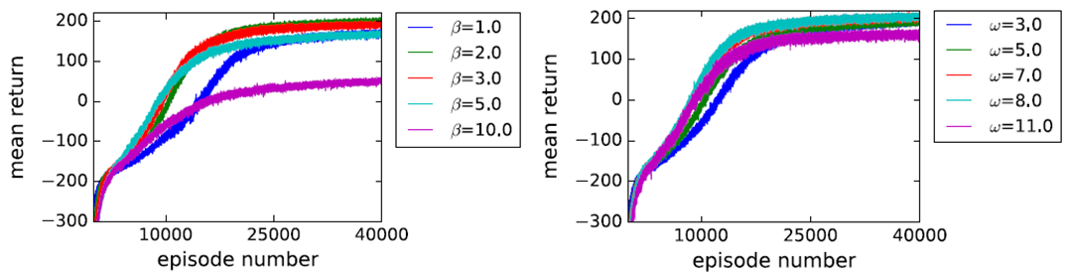
\includegraphics[scale=0.7]{lunar_paper1.png}\\
    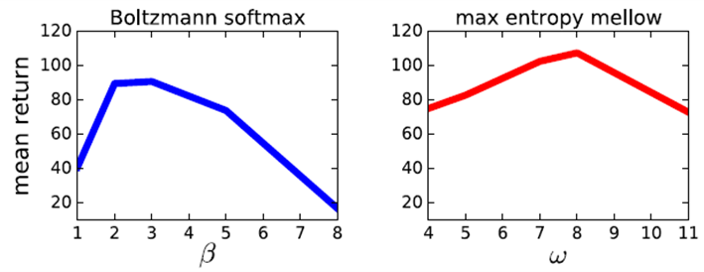
\includegraphics[scale=0.7]{lunar_paper2.png}
\end{center}
In the paper's results, the Boltzmann softsmax method performs well when $\beta=2, 3$, and the Mellowmax method 
performs well when $\omega=7, 8$.The Boltzmann softmax method, $\beta=10$ performs the worst in the 10 experiments, it 
gets a much lower average mean return than others.The Mellowmax method, $\omega=8$ performs the best in the 10 experiments.\\\\
Our results:\\
\begin{center}
    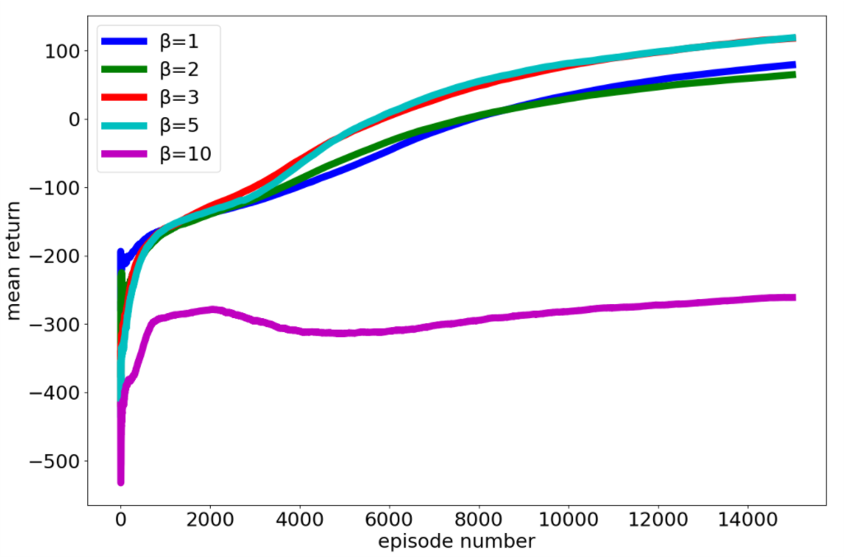
\includegraphics[scale=0.4]{lunar_rep1.png}
    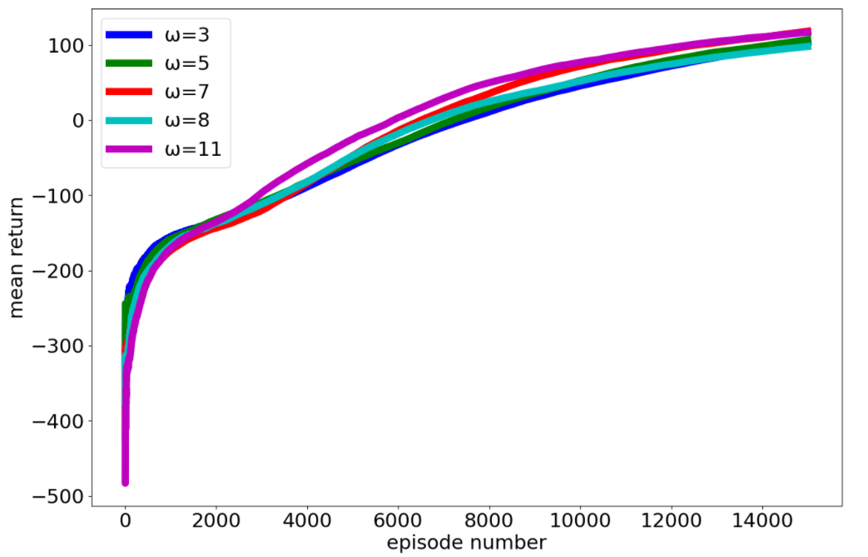
\includegraphics[scale=0.4]{lunar_rep2.png}\\
    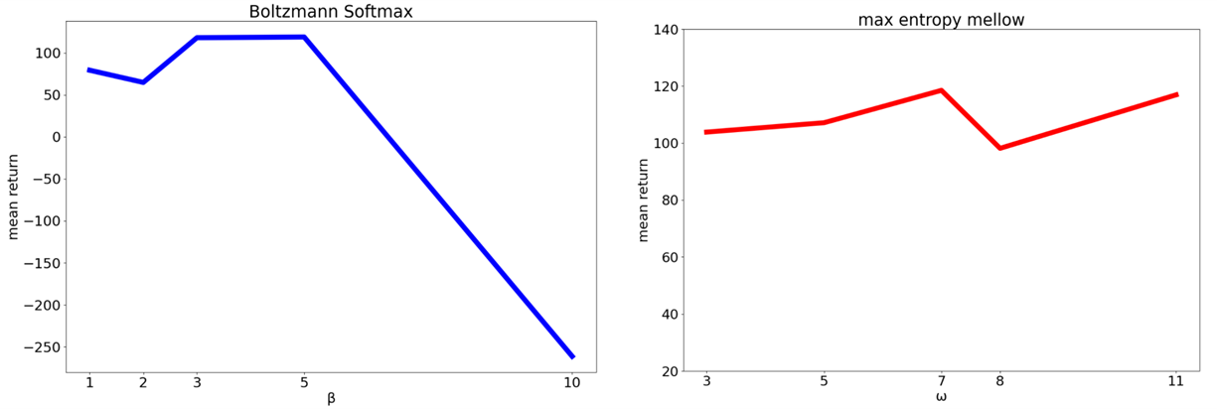
\includegraphics[scale=0.6]{lunar_rep3.png}
\end{center}
In our results, the Boltzmann softmax method performs well when $\beta=3, 5$, and the Mellowmax method 
performs well when $\omega=7, 11$. The Boltzmann softmax method, $\beta=10$ performs the worst in the 10 experiments and
gets a much lower average mean return than others. The Mellowmax method, $\omega=7$ performs the best in our 10 experiments.\\\\
\subsection*{Comparison}
Our experiment results are a little different from the paper's, and we think it is because that we use much less runs and less episodes in each run.
The mean return of Boltzmann softmax $\beta=10$ is about -300, and it's much lower than the paper's result. We find that it gets a lot of negative
 rewards at seed=22, its ewma reward is less than -1000 during almost all episodes, however, its ewma reward reaches 200 while seed=7654.
It seems that Boltzmann softmax $\beta=10$ is unstable, so the chosen seed affects a lots, and more runs are needed to get precise results.


\section{Conclusion}
\label{section:conclusion}
The whole survey and replication through the paper could summarize the advantages of Mellowmax in the following points:
\begin{itemize}
\item The non-expansion property: the convergence of GVI is guaranteed
\item more stable during the training
\end{itemize}
and the disadvantages of Mellowmax is that:
\begin{itemize}
\item Using Mellowmax operator may need more time to solve beta, but may get better updates during training.
In LunarLander, it takes about 0.0014 sec per step with Boltzmann softmax and 0.0046 sec per step with Mellomax.
\end{itemize}
This paper proposed the Mellowmax operator as an alternative to the Boltzmann softmax operator. We also replicated that mellowmax has several desirable properties and that it works favorably in practice. Arguably, mellowmax could be used in place of Boltzmann throughout reinforcement-learning research.


{
\small
\bibliographystyle{unsrtnat}
\bibliography{reference}
}


\end{document}
